% Generated by thesis/ch7/exp2/networks.py -- do not edit by hand.
\begin{sidewaysfigure}
  \centering
  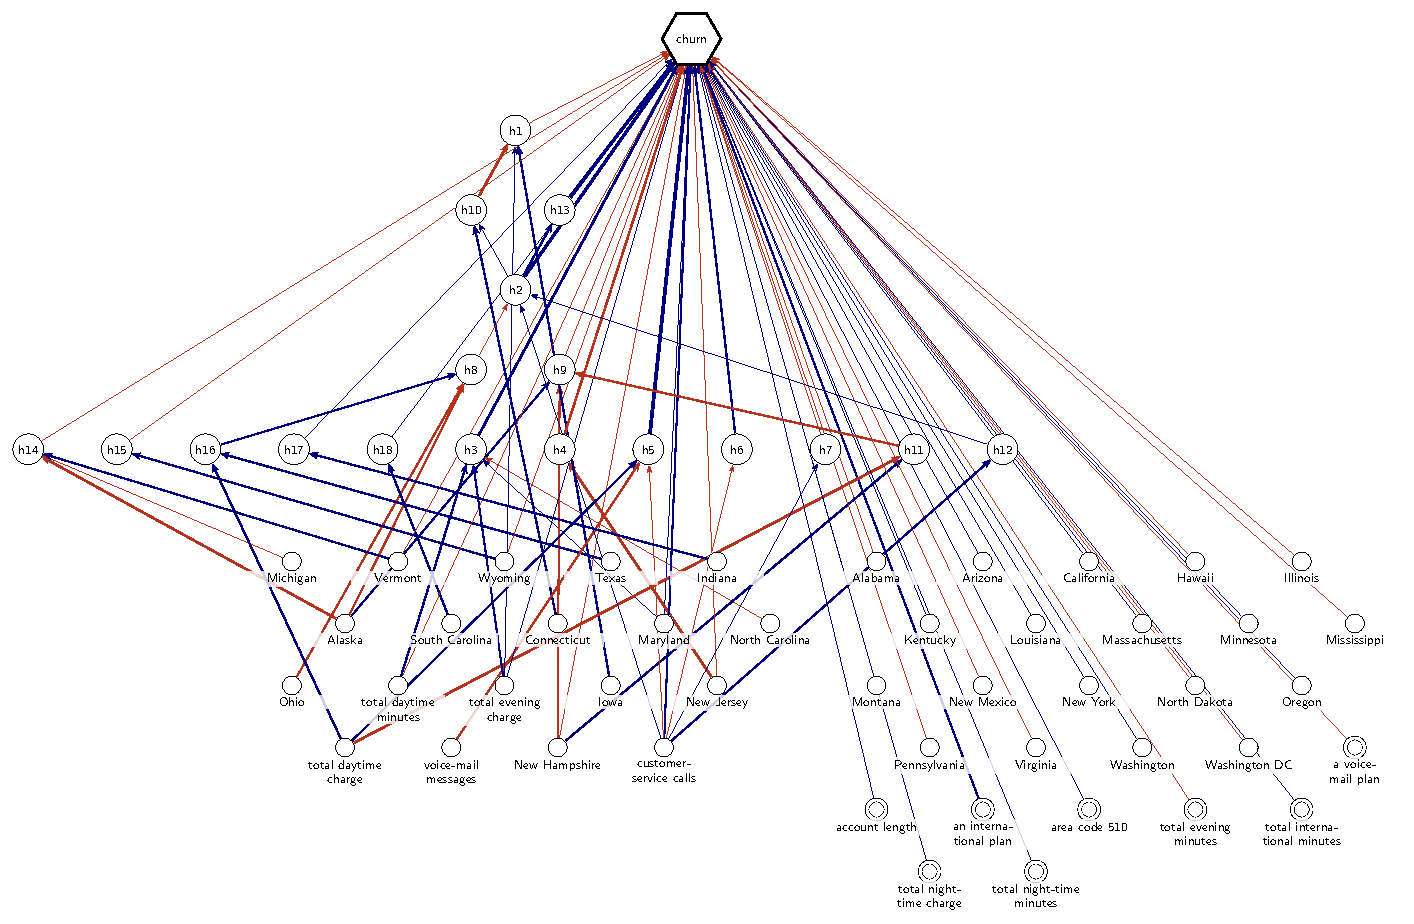
\includegraphics[width=\textheight,height=0.78\textwidth,keepaspectratio]{figures/exp2/networks/churn100-s6-raw}
  \caption{Churn, seed 6 (churn100-s6): the network as trained, before any explanation, in full. Inputs at the bottom (every input column its own node), hidden units by depth, the output at the top; 46 of 71 input columns are connected, with 18 hidden units and 84 enabled connections. Blue: positive weight (raises the score); red: negative weight (lowers it); thicker: larger weight. Orange outline and up arrow: raises the final prediction; teal and down arrow: lowers it; grey and double arrow: depends. Not used (no connection; 25 columns): Georgia, Idaho, Kansas, Arkansas, Maine, Missouri, Nebraska, Nevada, Oklahoma, Rhode Island, South Dakota, Tennessee, Utah, Wisconsin, West Virginia, Colorado, Delaware, Florida, area code 408, area code 415, total daytime calls, total evening calls, total night-time calls, total international calls and total international charge.}
  \label{fig:exp2-net-churn100-s6-raw}
\end{sidewaysfigure}
